% theKATRINexperiment.tex
%

    \chapter{KATRIN experiment}
    \label{ch:The KATRIN experiment}
    The KATRIN experiment is on its way to measure the neutrino mass or set new upper limits at precisions never achieved before. It will reach a sensitivity of \SI{200}{\milli\electronvolt}/\SI{}{\square c} at \SI{90}{\percent} C.L. excelling the previously best experiments of Mainz and Troisk by a factor of \SI{10}{}. Major challenges of the project are the requirement of ultra high vacuum, the exact knowledge of all magnetic and electric fields as well as external influences on those, the required high luminosity of the tritium source and the classification and reduction of background sources.
    
      \section{Measurement principle}
      \label{ch:The KATRIN experiment:sec:Measurement Principle}
      A generally easy principle is used to find information on the neutrino mass: The energy of electrons from tritium decay is measured with high precision and compared to the standard model's presumption for a massless neutrino: 
      \begin{equation}
      	\ce{^3_1T -> ^3_1H^+ + e^- + \bar{\nu}_e}
      \end{equation}
      As the decay's energy is distributed between the constant neutrino's rest mass and its and the electron's kinetic energies respectively, the decay electrons will show a continuous spectrum. The difference between the electron energy calculated by standard model presumptions to the extrapolated maximum electron energy from the spectrum then equals the neutrino rest mass as shown on figure \ref{fig:katrinExperiment:tritiumSpectrum}
      \begin{figure}
	\centering
      	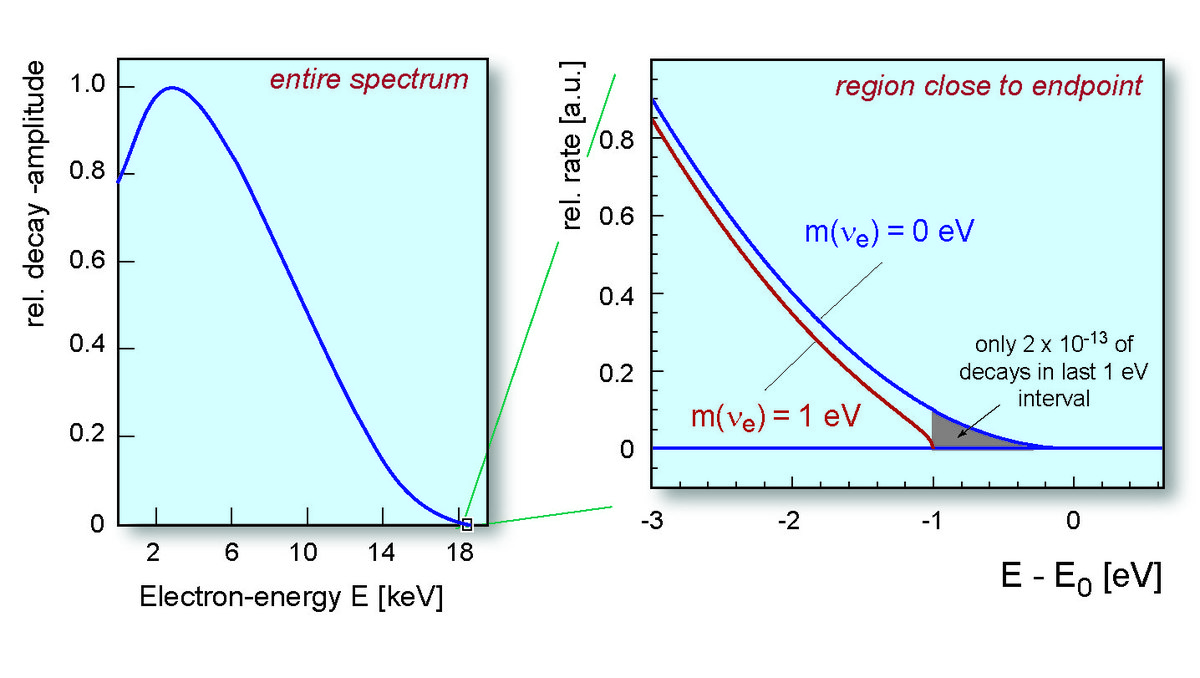
\includegraphics[width = 0.9 \textwidth]{graphics/katrinExperiment/electronSpectrum.jpg}
      	\caption[Schematic tritium energy spectrum]{Schematic energy spectrum for electrons from tritium beta decay. On the left, the entire spectrum with the peak at the energy most emitted - around \SI{5}{\electronvolt} - can be seen. On the right, a zoom-in on the endpoint showing both the calculations for a massless and a \SI{1}{\electronvolt} neutrino. As described in the graph, rates in this region are extremely low and extrapolation through advanced software tools needs to be applied.}
      	\label{fig:katrinExperiment:tritiumSpectrum}
      \end{figure}
      A different light is shed on the simplicity of the task when considering the needed accuracy of 

      \section{Experimental Setup}
      \label{ch:The KATRIN experiment:sec:Experimental setup}
      The KATRIN experiment is made up of different section all fulfilling their own important purpose in the whole setup. We start off with the production of tritium electrons in the very south. These are guided magnetically northwards through pumping tracks removing hydrogen ions and other residual gases in the process on through the two spectrometers posing as a energetic high pass filter to the focal plane detector registering them. See figure \ref{fig:beamLine} for a schematic overview. It follows a more detailed description of the single components.
      
      \begin{figure}
			
      		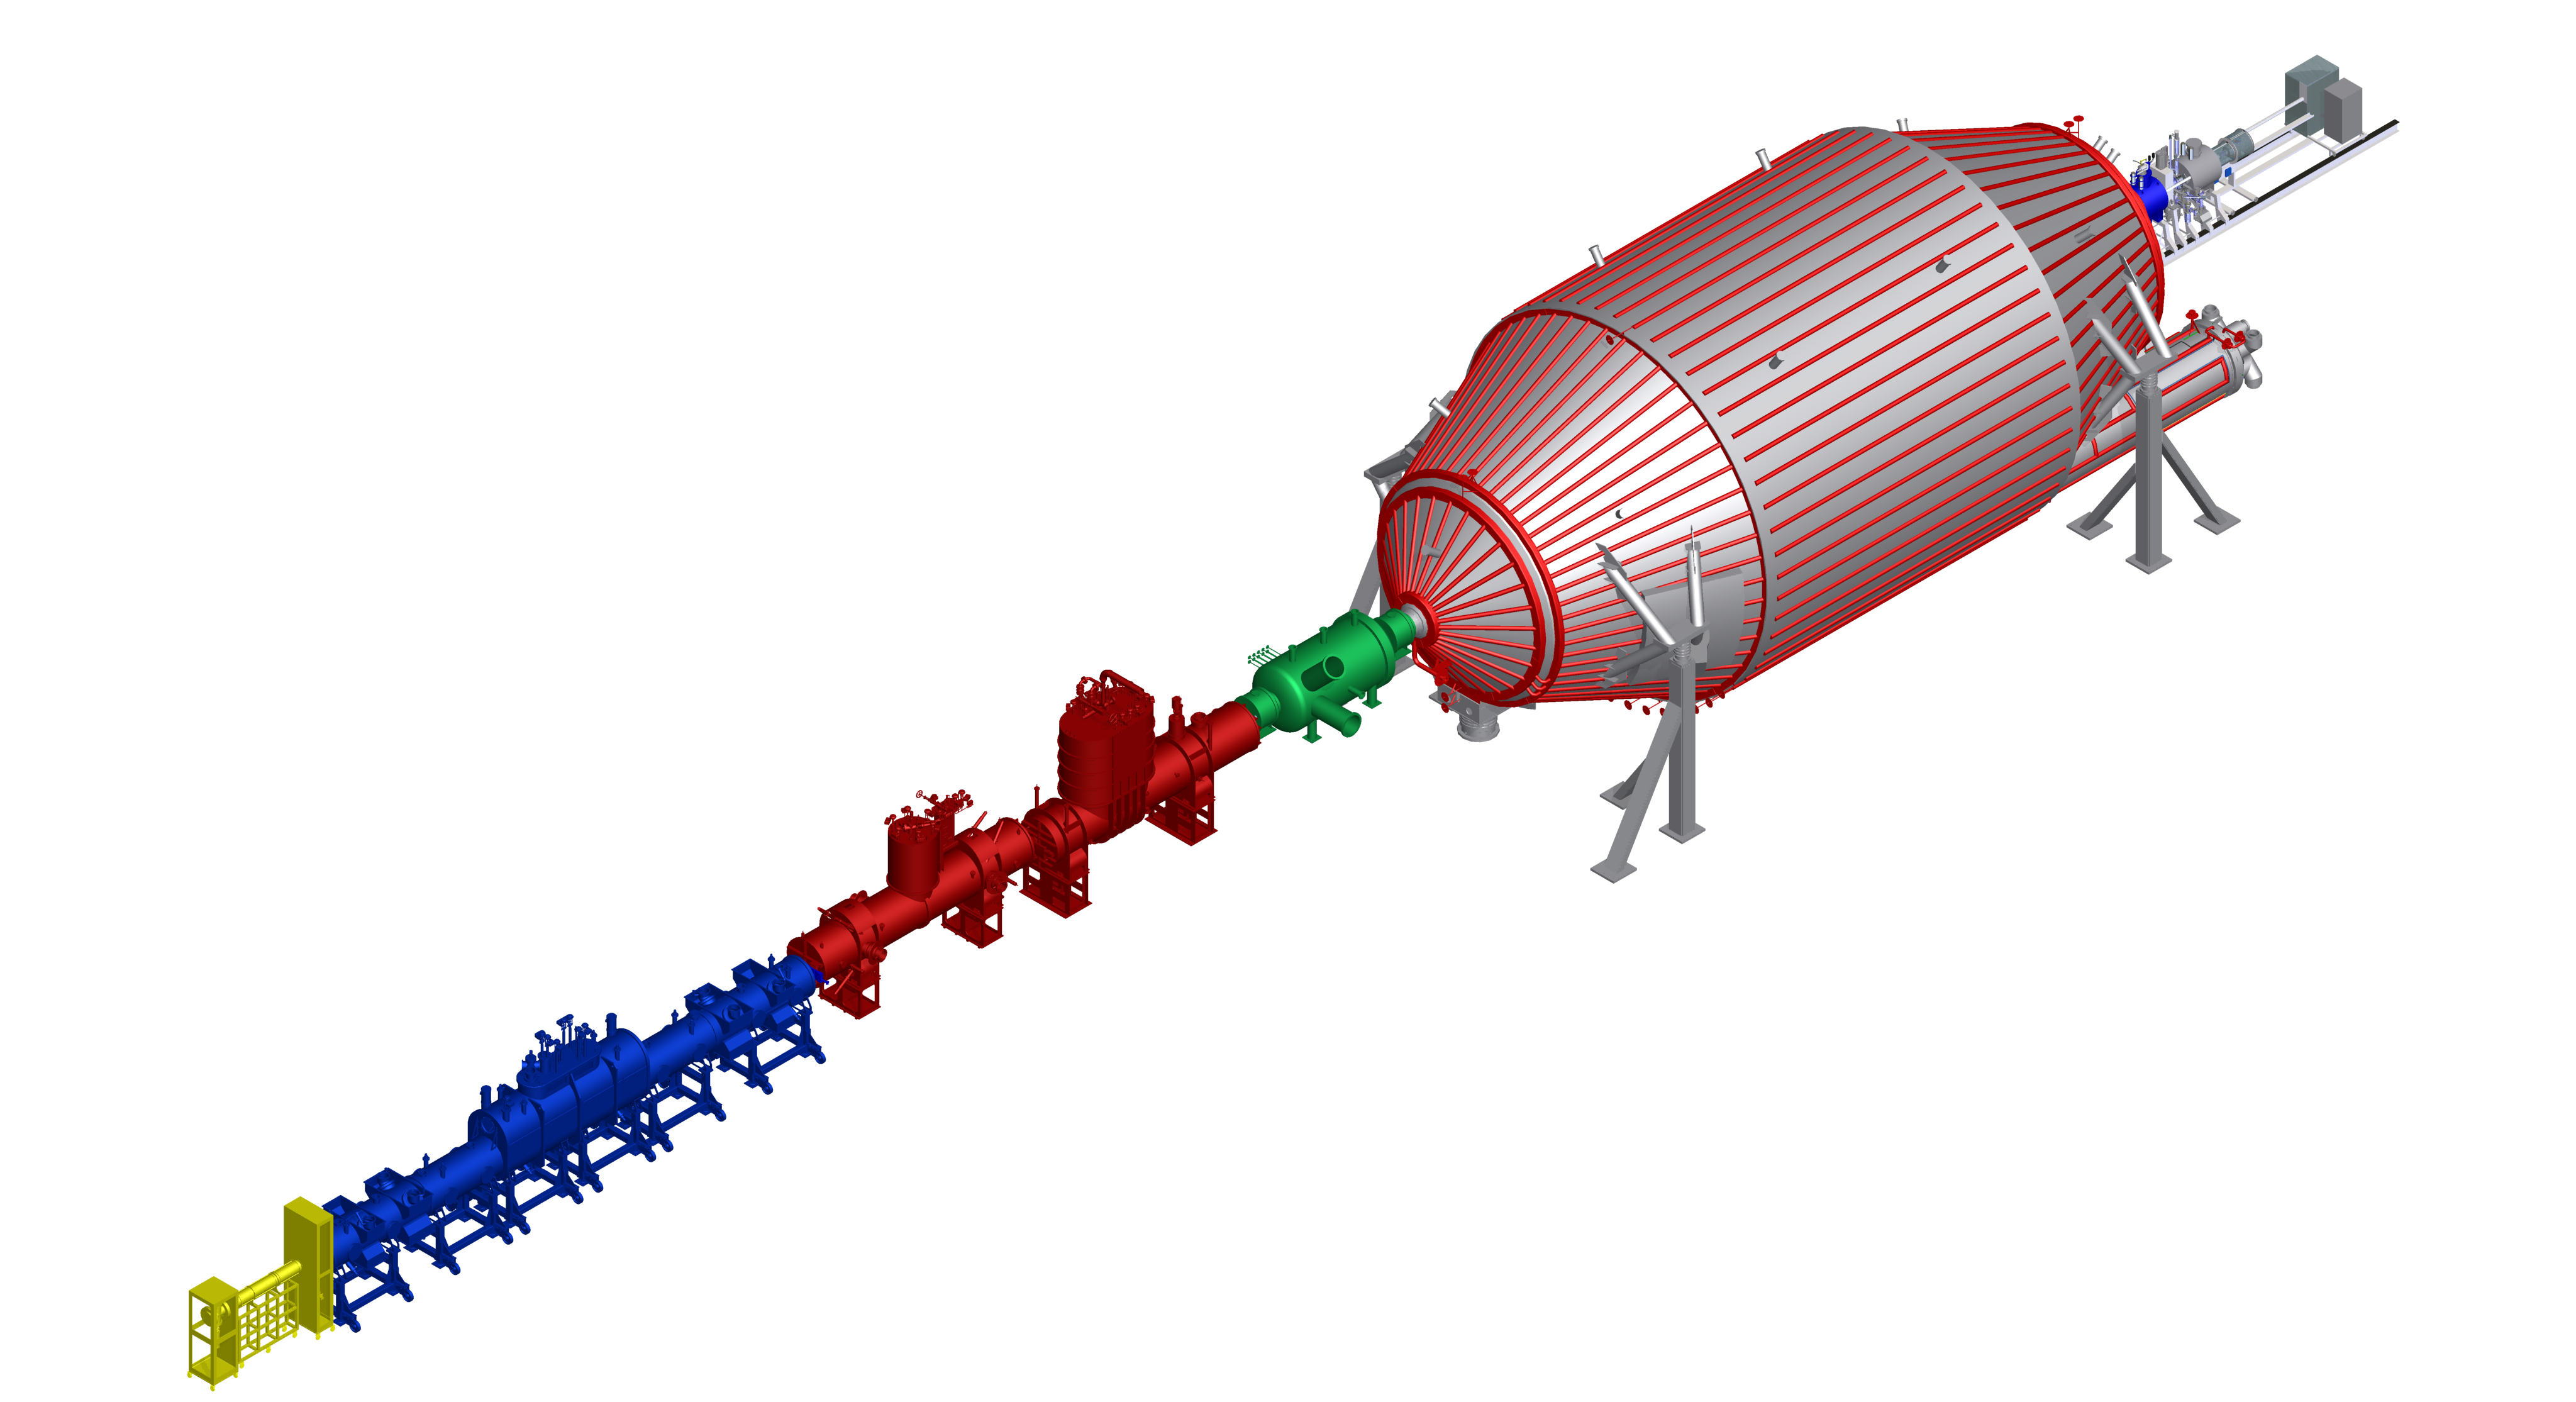
\includegraphics[width = \textwidth]{graphics/katrinExperiment/beamLineHD.jpg}

      	\caption[KATRIN beam line]{The beam line of the KATRIN experiment with the different stages: Rear section (yellow) and WGTS (blue) on the very left, followed by the transport section (red) consisting of DPS and CPS. Energy analysis in pre- (green) and main spectrometer (grey) of the spectrometer section and electron detection at the detector section (grey, upper right).}
      	\label{fig:beamLine}
      \end{figure}

      
      \subsection{Source and Rear Section}
      \label{ch:The KATRIN experiment:sec:Experimental setup:subsec:sourceSide}
      The required high luminosity is achieved by using a gaseous Tritium source. In a solid, most electrons from decays inside the structure would be resorbed quickly and be unavailable for analysis. The gas's large advantage is that not only the surface facing the detector emits electrons at the desired spectrum, but the whole volume covered by the magnetic flux tube arriving at the detector can be utilized. Of course, new challenges arise from the decision to use gas instead of solids: The spectrometers further downstream require for ultra high vacuum, for the main spectrometer in the order of \SI{e-11}{\milli\bar}. As the Tritium pressure is in the order of \SI{10e-3}{\milli\bar} and the source needs to be windowless - as no electron transparent window is known to stand such pressure differences - the pressure must be reduced to desired values without any physical barrier. 
      For that purpose, after being allowed to decay inside the WGTS, the windowless gaseous tritium source, electrons fly on through DPS and CPS, the differential- and cryogenic pumping sections. 
      
     \begin{figure}
		\begin{minipage}{0.7\textwidth}
				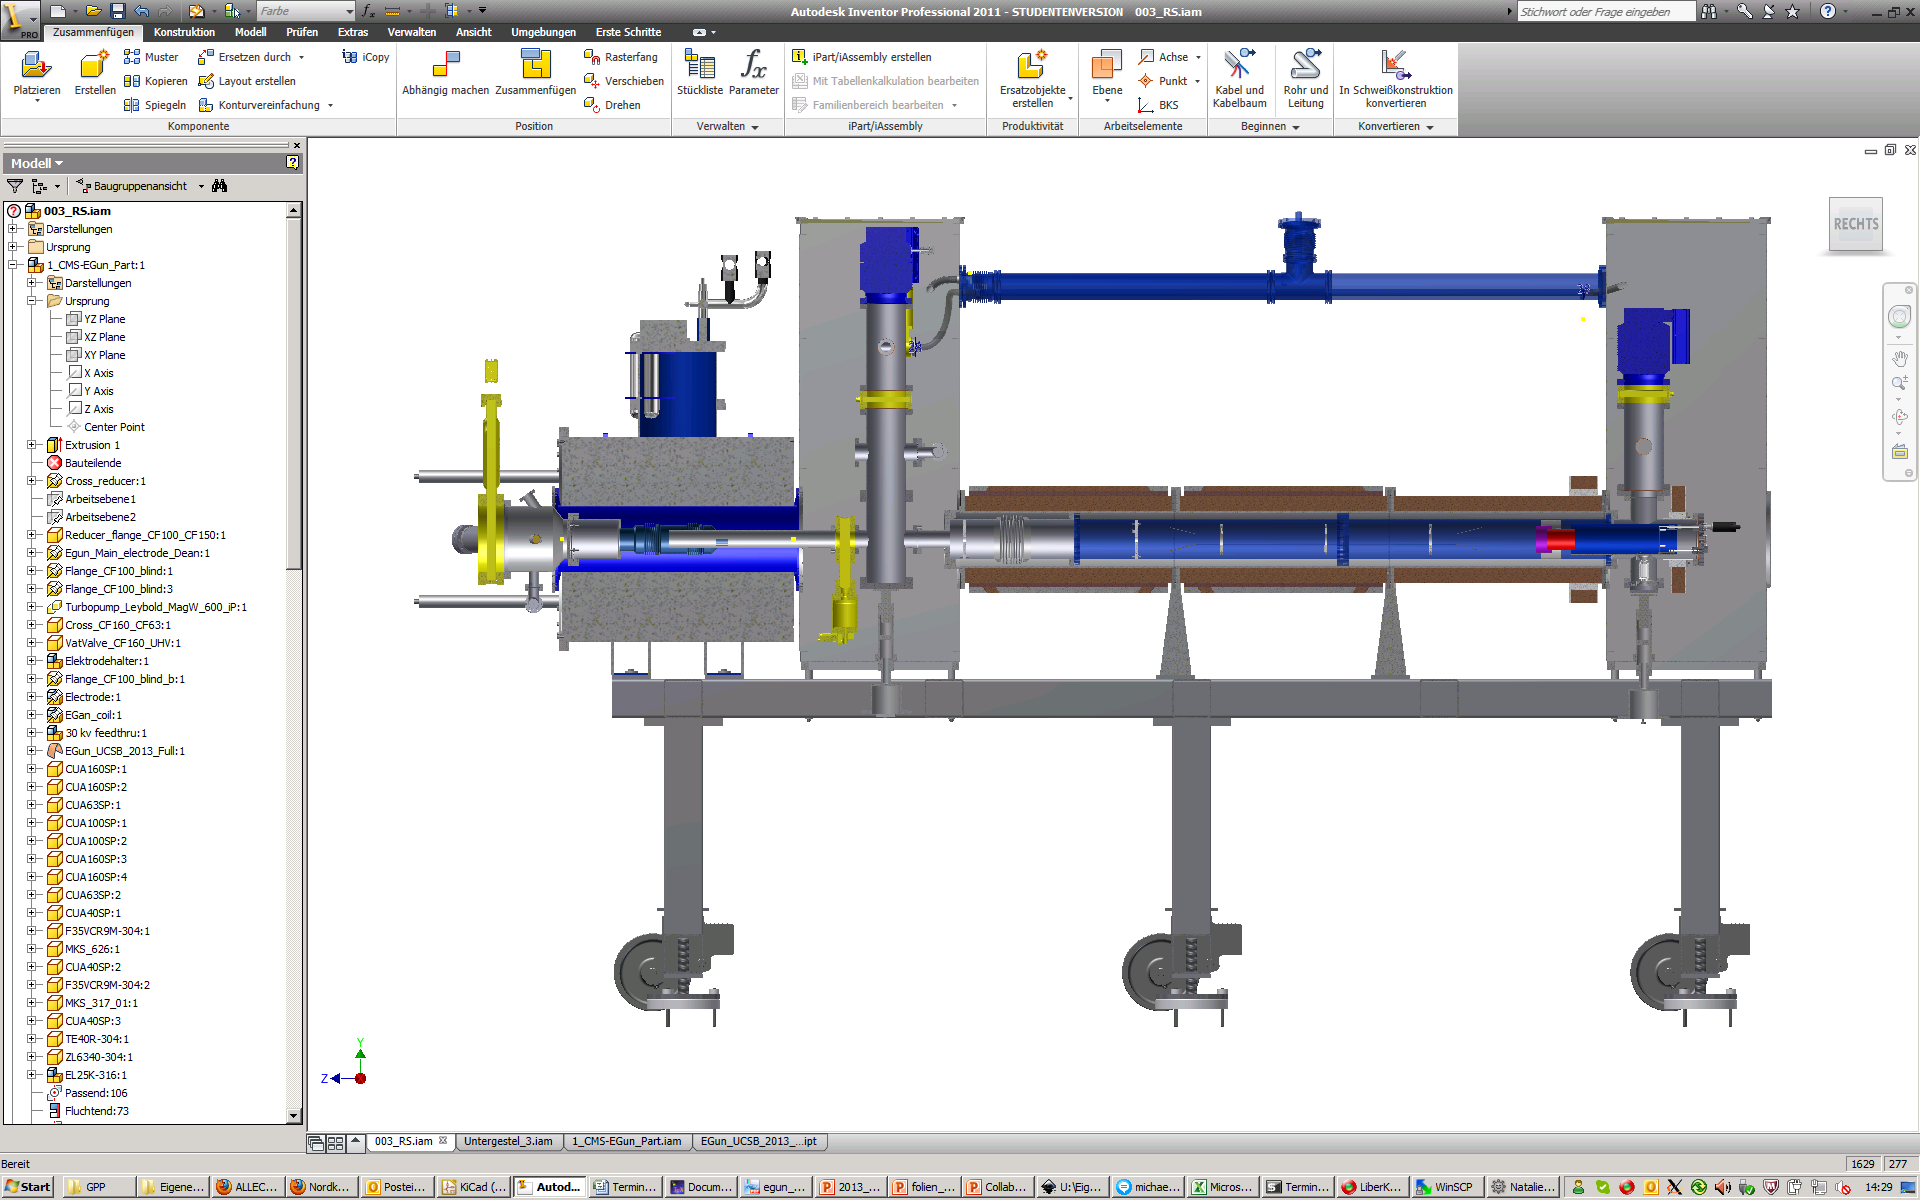
\includegraphics[width = 1.0\textwidth]{graphics/katrinExperiment/rearSection.png}
		\end{minipage}
		\begin{minipage}{0.7\textwidth}
			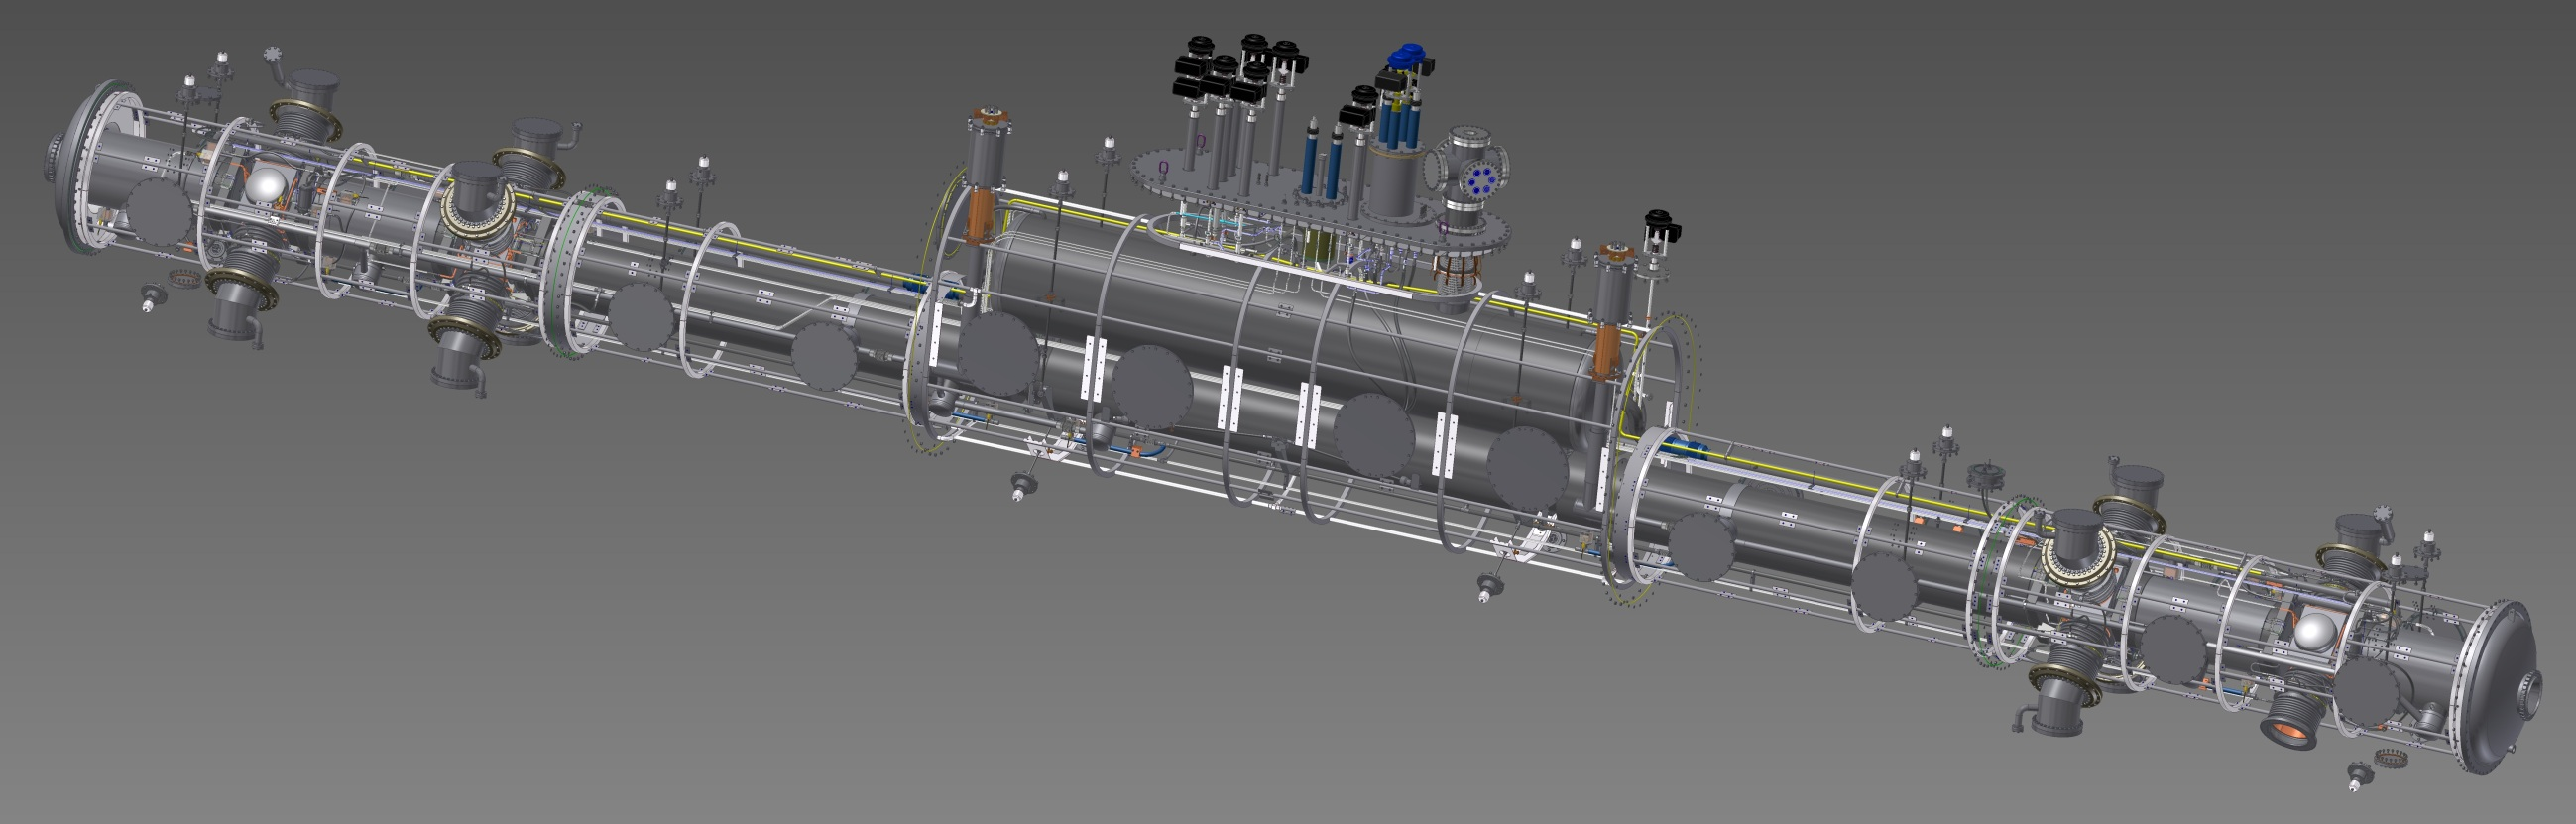
\includegraphics[width = 1.0\textwidth]{graphics/katrinExperiment/WGTS.jpg}
		\end{minipage}
		\caption[DPS and CPS]{Images from \cite{rearSection} and \cite{WGTSDrexlin}}
		\label{fig:sourceSide}
      \end{figure}
      
      
      \subsection{Transport and Pumping Section}
      
      In the DPS, pressure is actively reduced by the use of turbo pumps. These need to be tested thoroughly to withstand the constant radiation by tritium decays \cite{tritiumTests}. Afterwards, the CPS uses strongly cooled walls to freeze residual gas, always keeping the information carrying electrons away from those by magnetic guidance.
      \begin{figure}
		\begin{minipage}{0.49\textwidth}
				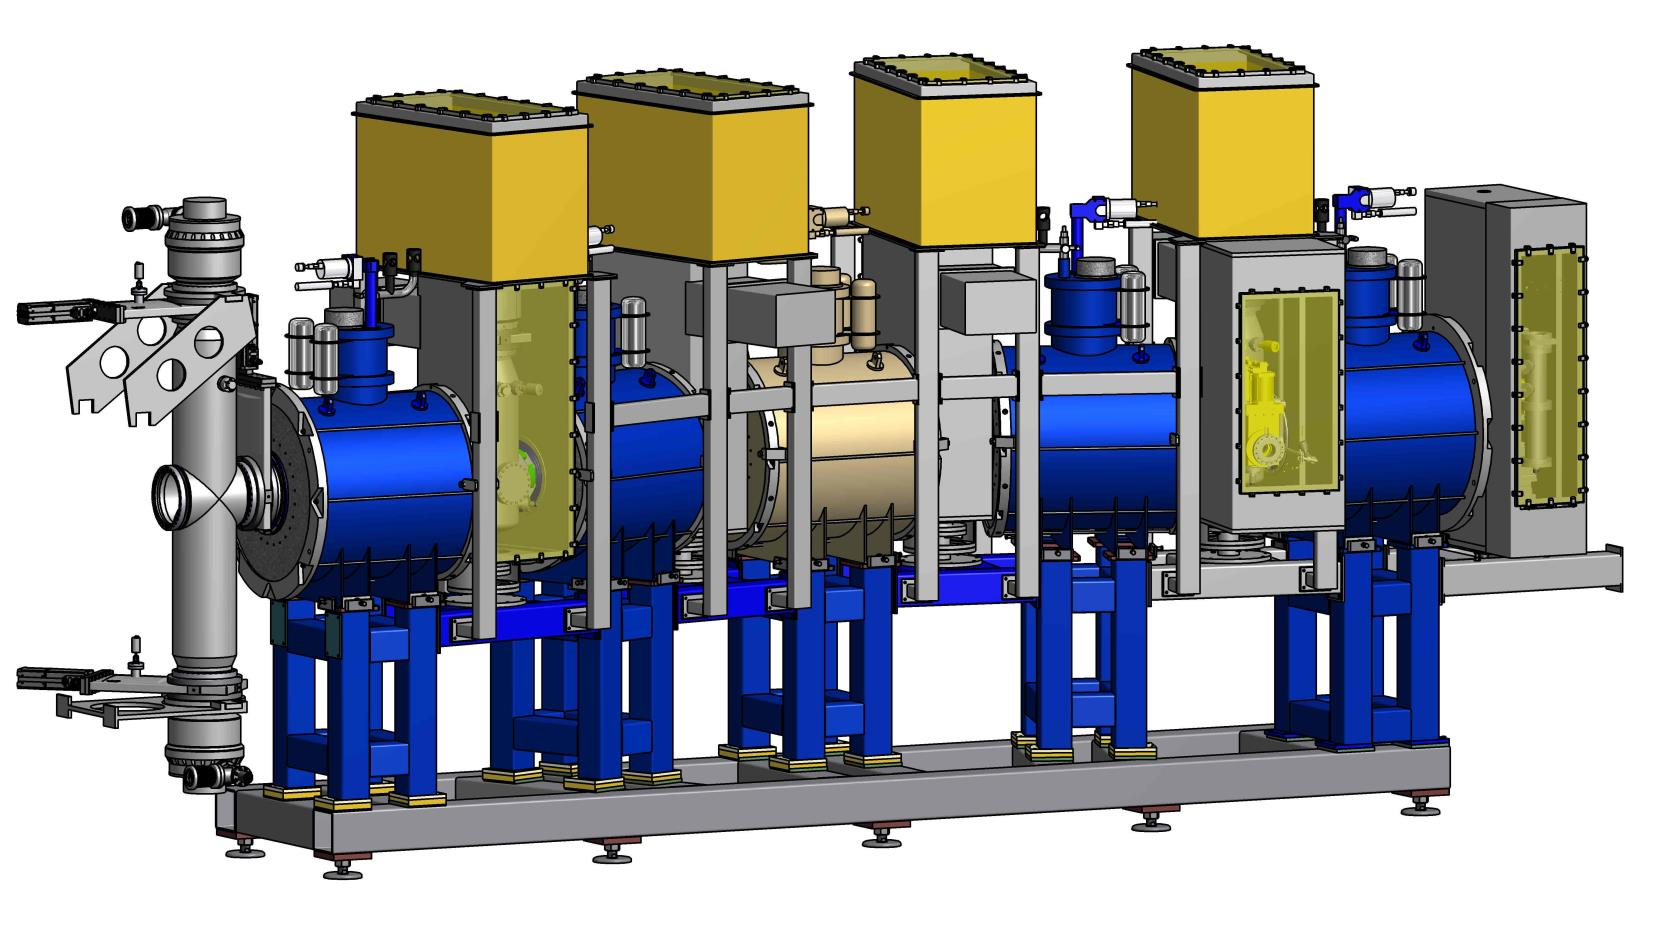
\includegraphics[width = 1.0\textwidth]{graphics/katrinExperiment/DPS.jpg}
		\end{minipage}
		\begin{minipage}{0.49\textwidth}
			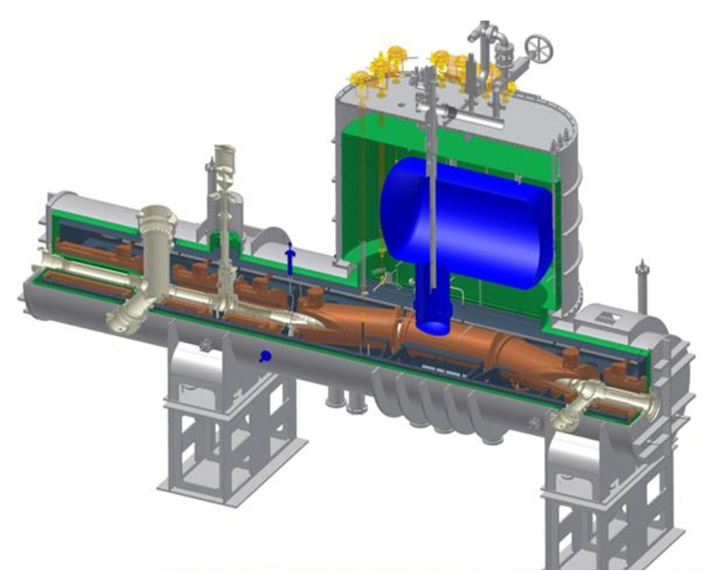
\includegraphics[width = 1.0\textwidth]{graphics/katrinExperiment/CPS.jpg}
		\end{minipage}
		\caption[DPS and CPS]{Differential and cryogenic pumping sections, left the DPS with pumping ports all over the structure. All of the ports are isolated against the surroundings (yellow boxes) to protect against potential radiation leaks. On the right the CPS with its coolable wall structure to capture free particle as well as standard pumping ports \cite{DPS, CPS}.}
      \end{figure}
      
      \subsection{Pre-Spectrometer}
      \label{ch:The KATRIN experiment:sec:Experimental setup:subsec:PreSpectrometer}
      The pre-spectrometer was built in Munster and works on the same principle as the main spectrometer, although being a lot smaller. It is installed to reduce the flux to the main spectrometer, and by that the possible amount of stored electrons inside the main vessel. The pre-spectrometer has a single layer of wires as a inner electrode to shield against externally induced electrons. It is made to 
      \subsection{Main Spectrometer}
      \label{ch:The KATRIN experiment:sec:Experimental setup:subsec:MainSpec}
      The largest component of all is the main spectrometer. With a diameter of \SI{9}{\meter} and a length of over \SI{24}{\meter}, it incorporates around \SI{1400}{\cubic\meter} that need to be evacuated to extremely high vacuum of < \SI{e-11}{\milli\bar}. The vessel is equipped with two layers of electrodes on a comb-like structure. This setup reduces the number of secondary electrons from the spectrometer walls entering the flux tube's volume. Keeping that count low, the rate of those electrons not reflected magnetically due to imperfect symmetries is reduced to the sub-\SI{}{\electronvolt} level. The layer made from thinner wires further to the inside shields the spectrometer volume from the one further towards the wall as cosmic rays may unleash electrons there as well.
      The main spectrometer as a whole is set to high voltage varied in the region below the endpoint of ~\SI{18.6}{\kilo\volt}. It constitutes the MAC-E filter from \ref{ch:The KATRIN experiment:sec:MAC-E}. The wire electrodes float on that voltage while being more negative to shield against electron background.
      \begin{figure}
      
      	\begin{minipage}{0.67\textwidth}
      		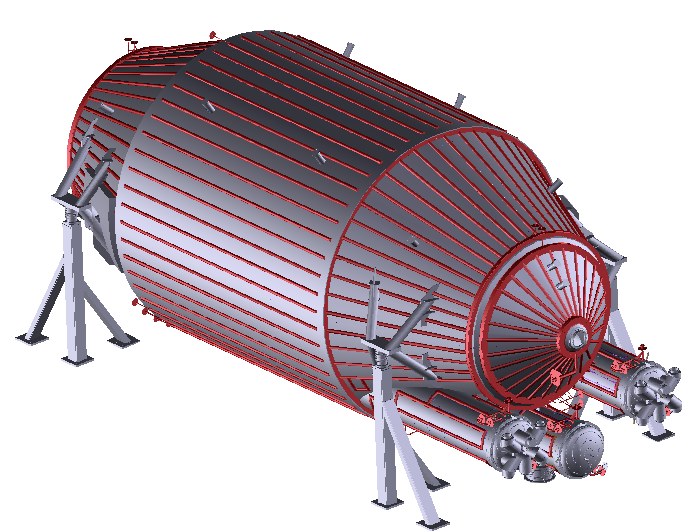
\includegraphics[width = \textwidth]{graphics/katrinExperiment/mainSpectrometer.jpg}
      	\end{minipage}
      	\begin{minipage}{0.29\textwidth}
      		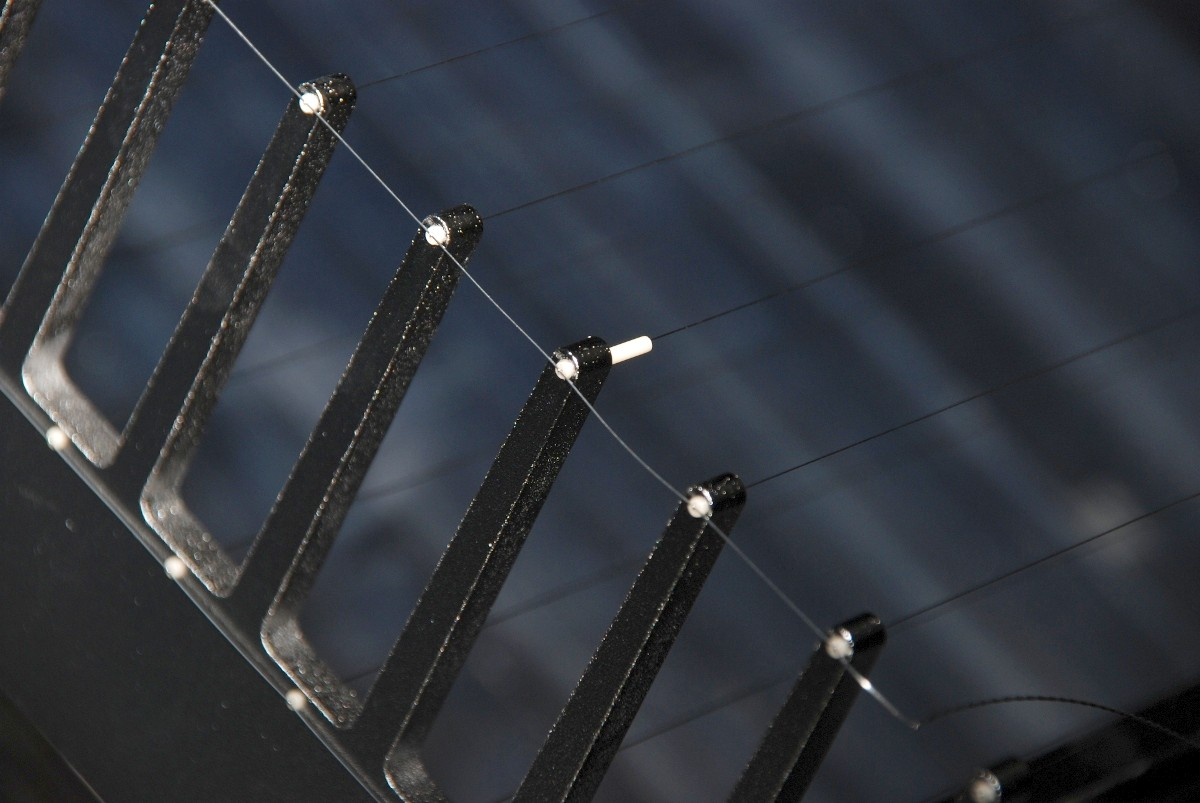
\includegraphics[angle = 90, width = \textwidth]{graphics/katrinExperiment/wireElectrodes.png}
      	\end{minipage}
      	\caption[Main spectrometer and wire electrodes]{On the left, the main spectrometer of the KATRIN experiment \cite{mainSpecStatus}. It is divided into a central, cylindric shape to which two flat cones, disemboguing in the steep cones, are attached. Also visible in this image are the 3 large pump ports on the lower right and the three-legged holding structures. On the right a image of the comb structure of the inner electrodes with both layers of wires visible. The white structures on both top and bottom of the combs are the insulation of the wires \cite{collabWireElectrodes}.}
      	\label{fig:mainSpec}
      \end{figure}
		
      \subsection{Monitor spectrometer}
      \label{ch:theKATRINexperiment:sec:experimentalSetup:subsec:monSpec}
      
      The monitor spectrometer is, next to the high precision voltage surveillance, a second tool to ensure the quality of the high voltage.

      \subsection{MAC-E Filter}
      \label{ch:The KATRIN experiment:sec:MAC-E}
      A high luminosity is a major requirement for good statistics at the KATRIN experiment. This makes it impossible to use some kind of aperture to filter for electrons from Tritium decay with one momentum direction as they are emitted uniformly from the source volume and the largest amount of electrons would never reach the main spectrometer. That is why another strategy is used at KATRIN: The MAC-E filter - magnetic adiabatic collimation with electrostatic filter - which utilizes the fact that, under small enough magnetic field changes, the magnetic momentum of a particle is constant; the particle can be considered adiabatic. The solenoid and coil system surrounding the main spectrometer are set up to create a strong, but smooth magnetic field gradient of several orders of magnitude. At entrance and exit of the vessel, solenoids generating fields of up to \SI{}{\tesla} are installed while in the central, widest part, the field strength reduces by a factor of \todo{factors and field strengths}. This area is called the analysing plane. According to
      \begin{equation}
      	\mu = \frac{E_{\bot}}{B} = const \propto \frac{p_\bot}{B}
      \end{equation}
      where $\mu$ is the magnetic momentum, $E_\bot$ the kinetic energy transversal to the field line and $B$ is the magnetic fields magnitude, the momentum will align with the magnetic field lines as the field weakens. In the edge case of $B\rightarrow 0$ in the analysing plane, the momentum would need to be exactly parallel to the field as the transversal motion would approach 0 as well. 
      One can not differentiate between electrons emitted parallel to a magnetic field line and those emitted under the maximum angle towards it as the filter is not a perfect one. So, following
      \begin{equation}
      	\mu_{\mathrm{0}} = \mu_{\mathrm{low}} ~ \longrightarrow ~ \frac{E_{\bot_0}}{B_0} = \frac{E_{\bot_{low}}}{B_{low}} 
      \end{equation}
      the energy resolution can be described by the field values, the electron's initial energy $E_0$ and its maximum transversal energy $E_{\bot_{max}}$ to be accepted by the filter:
      \begin{equation}
	    \Delta E = E_{\bot_{max}} = E_{\bot_0}\frac{B_{low}}{B_{0}}
      \end{equation}
      The main spectrometer reaches a resolution of \SI{0.93}{\electronvolt}.
      To further filter out electrons with high starting angle, the source is set to lower fields than the maximum $B_{max}$.
      As with larger angles come longer paths, this reduces the probability of electrons taking part in scattering processes inside the source section being detected.
      \begin{equation}
      	\theta_{s~max}= \arcsin{\sqrt{\frac{B_s}{B_{max}}}}
      \end{equation}
      With the chosen settings This results in an angular acceptance of 2$\pi$.
      
            \begin{figure}
	\centering
      	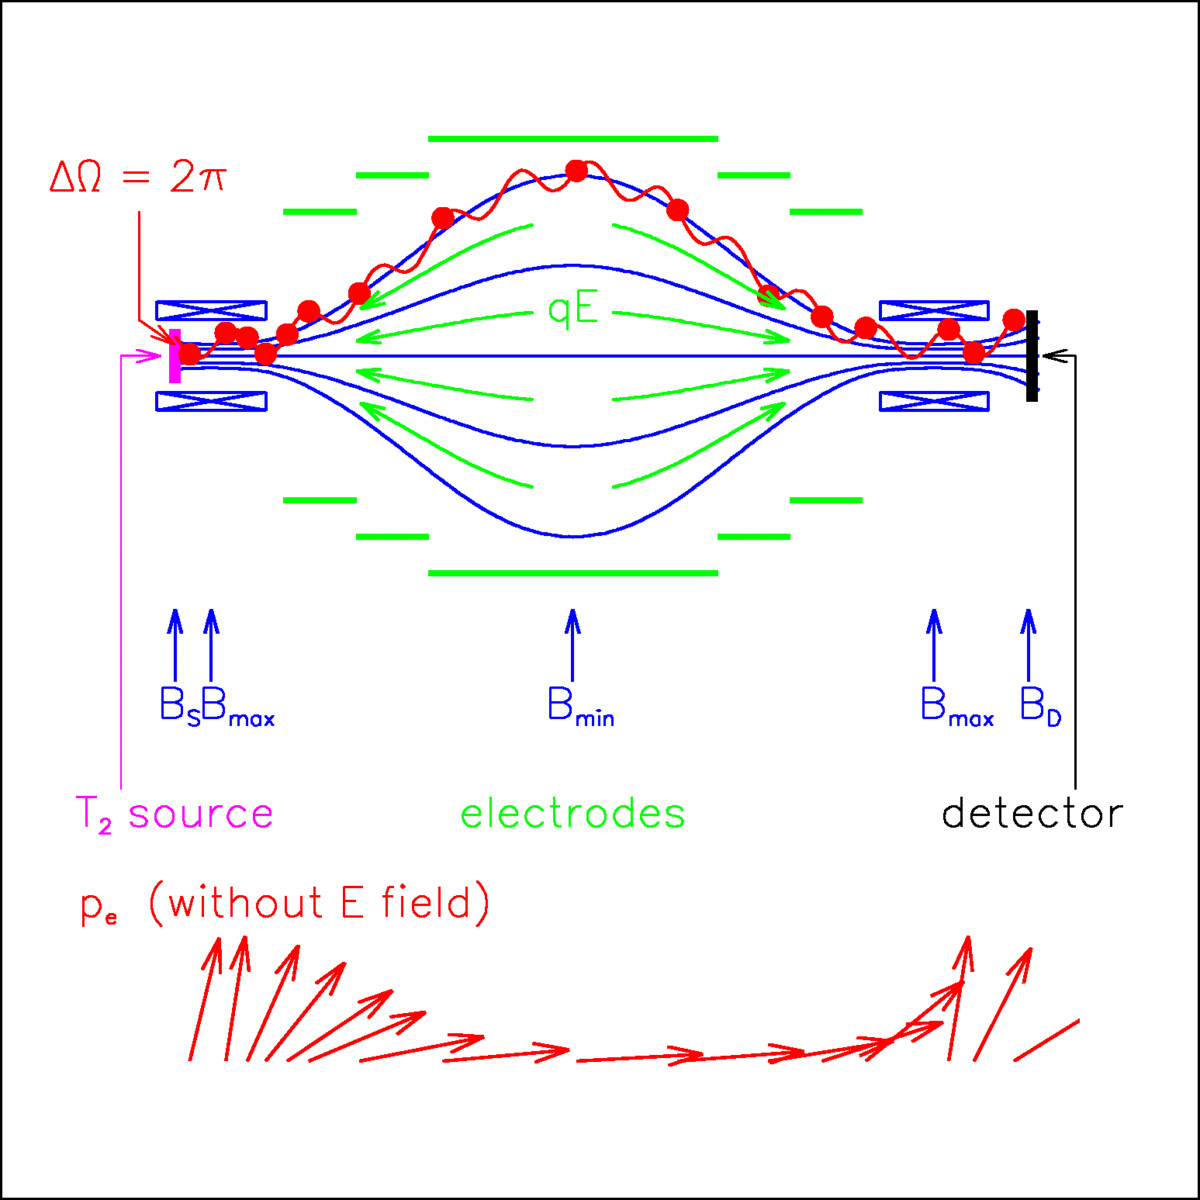
\includegraphics[width = 0.6 \textwidth]{graphics/katrinExperiment/macEFilter.jpg}
      	\caption[MAC E Filter]{Functionality of a MAC E filter. The angular momentum of an electron not starting parallel to the magnetic field lines is converted mostly to linear kinetic energy up to the point of lowest fields. Here, the energy is analyzed before the particle is guided towards the detector \cite{macEFilter}.}
      	\label{fig:katrinExperiment:macEFilter}
      \end{figure}
      
      \subsection{Focal Plane Detector System}
      \label{ch:The KATRIN experiment:sec:Experimental setup:subsec:FPD system}
      The main detector is located at the very north of the experiment. It is made up of a silicon wafer divided into 148 pixels attached to the readout electronics by pin connectors. The pattern is dartboard-like, multiple pixels with the same distance to the center form rings. Every pixel has the same surface area, making rates more easily comparable - that is if the magnetic flux through the wafer is as homogeneous as in this experiment.
      The detector system is roughly divided into two chambers: one connected to the ultra high vacuum of the main spectrometer and one with a lower grade vacuum on the detectors readout side.
      
      
      \begin{figure}
      \centering
	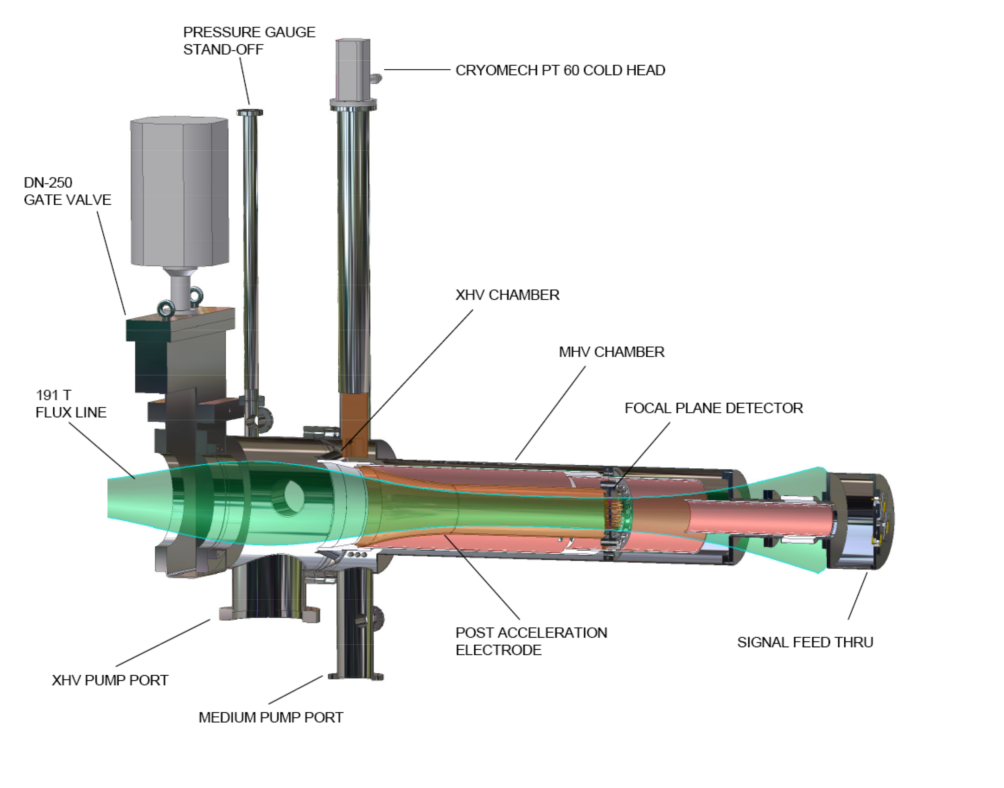
\includegraphics[width = 0.8 \textwidth]{graphics/katrinExperiment/detectorHousing.pdf}
	\caption[Focal plane detector system]{The focal plane detector system including the flux tube (green). One can make out the different grade vacuum sections: extremely high vacuum (XHV) and medium high vacuum (MHV). The post acceleration electrode is visible left of the actual detector and its signal feed trough on the very right. Multiple flanges and connectors are shown, not in this image are the calibration source holders \cite{FPD}.}
	\label{fig:katrinExperiment:detectorHousing}
      \end{figure}
      
      \begin{figure}
%       	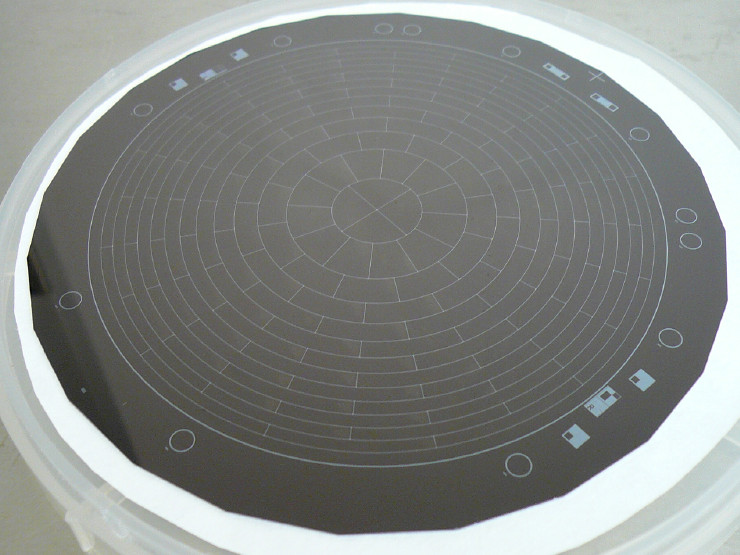
\includegraphics[width = 0.9 \textwidth]{graphics/katrinExperiment/detectorWafer.pdf}
	  \caption[Detector wafer]{The detector wafer as installed in the FPD system. Note the ``dartboard pattern'' with the four pixel bullseye in the center on the left side.}
	  \label{fig:katrinExperiment:detectorWafer}
      \end{figure}
      
      
      For background reduction, the detector system features both a passive shielding and an active veto system read out by the same data crate as the detector itself. It allows to discriminate externally triggered events. due to the high magnetic fields from detector and pinch magnet, semiconductor readout electronics had to be used instead of conventional photomultiplier tubes.
      As it may be necessary to investigate electrons with energies below the detector threshold, especially for background investigations, a post acceleration electrode has been installed - also visible in \ref{fig:katrinExperiment:detectorHousing} that can raise the energies through an electric field of known strength.
      \subsection{Solenoids, LFCS and EMCS system}
      \label{ch:The KATRIN experiment:sec:Experimental setup:subsec:Solenoids, LFCS and EMCS system}
      
      To achieve magnetic guidance in the way explained above, a sophisticated system of superconducting solenoids, the low field correction system LFCS and the earth magnetic field compensation system EMCS have been installed \cite{airCoilSystem}. These make sure that the path of flight is kept away from the wall and can be considered adiabatic, that penning traps are avoided as far as possible, that the earth magnetic field is compensated for and, most importantly, that the field drop to the analysis plane is of the order of \todo{order?} so the spectrometers resolution will achieve desired values.
      

      \subsection{Background sources}
      \label{ch:The KATRIN experiment:sec:Experimental setup:subsec:BackgroundSources}
      Different sources contribute to the background of electrons arriving at the detector. First, there is background due to stored electrons \cite{storedElectrons}. Penning traps cause electrons with fitting energies to be trapped in a potential cup. Discharges of those traps due to scattering processes with either residual gas or due to excessive filling of the trap can cause high-rate events at the detector. This can be both dangerous for the detector itself as it is harmful for data taking. Stored electrons can be both from external sources as from within the spectrometer. Decays of residual gas or wall absorbed molecules can contribute to the background. One large background source is radon, a neutral particle enabling it to move freely inside the vessel. Radon alpha decays, but shakeoff-, conversion- and auger electrons can then be guided to the detector \cite{radonGoerhard}.
      
      Another large background source are cosmic rays interacting with the vessel hull and producing electrons like that. This background is reduced mainly by two factors, one: the symmetry of the magnetic field and two: the wire electrodes shielding the flux tube up to a certain threshold energy.
      To one: if the fields, both electric and magnetic, were perfectly symmetrical and parallel, only particles generated within the flux tube would be guided towards the detector. But through inhomogeneities and alignment errors, electrons may enter the flux tube even if generated externally, e.g at the spectrometer wall through $E\times B$ drifts. To keep this from happening, point two, the wire electrodes, were installed. They shield the flux tube against electrons with energies up to $E_e = U_{wire}e$ depending on the wire electrodes voltage $U_{wire}$. 